\section{Data partitioning}

The spatial indices structure can be derived either from one-dimensional structures (such as a grid file) or from ad-hoc structures (like an R-tree), resulting in a myriad of potential data structures.

\paragraph*{Classification}
Spatial indices can be classified based on:
\begin{itemize}
    \item \textit{Type of objects}: points, lines, and regions. 
    \item \textit{Type of subdivision}: 
        \begin{itemize}
            \item Space partitioning: splits are executed according to global considerations, which is beneficial for uniform distributions and easier to implement.
            \item Data partitioning: splits are performed based on local considerations, akin to B+-trees. 
                This method is suitable for arbitrary distributions but is more complex to implement.
        \end{itemize}
    \item \textit{Type of organization}: either tree-based or hash-based. 
\end{itemize}
The prevalent approach involves organizing space into regions, referred to as cells, where each cell corresponds to a data page (although this correspondence is not always one-to-one).

\subsection{Grid files}
The Grid file arranges the spatial domain into a grid, with each dimension divided into intervals of arbitrary sizes. 
This entails the use of $d$ scales (monodimensional arrays) that hold values serving as separators for each dimension. 
Each grid cell is linked to a data page on disk, allowing for the possibility of two or more cells sharing the same data page.
\begin{figure}[H]
    \centering
    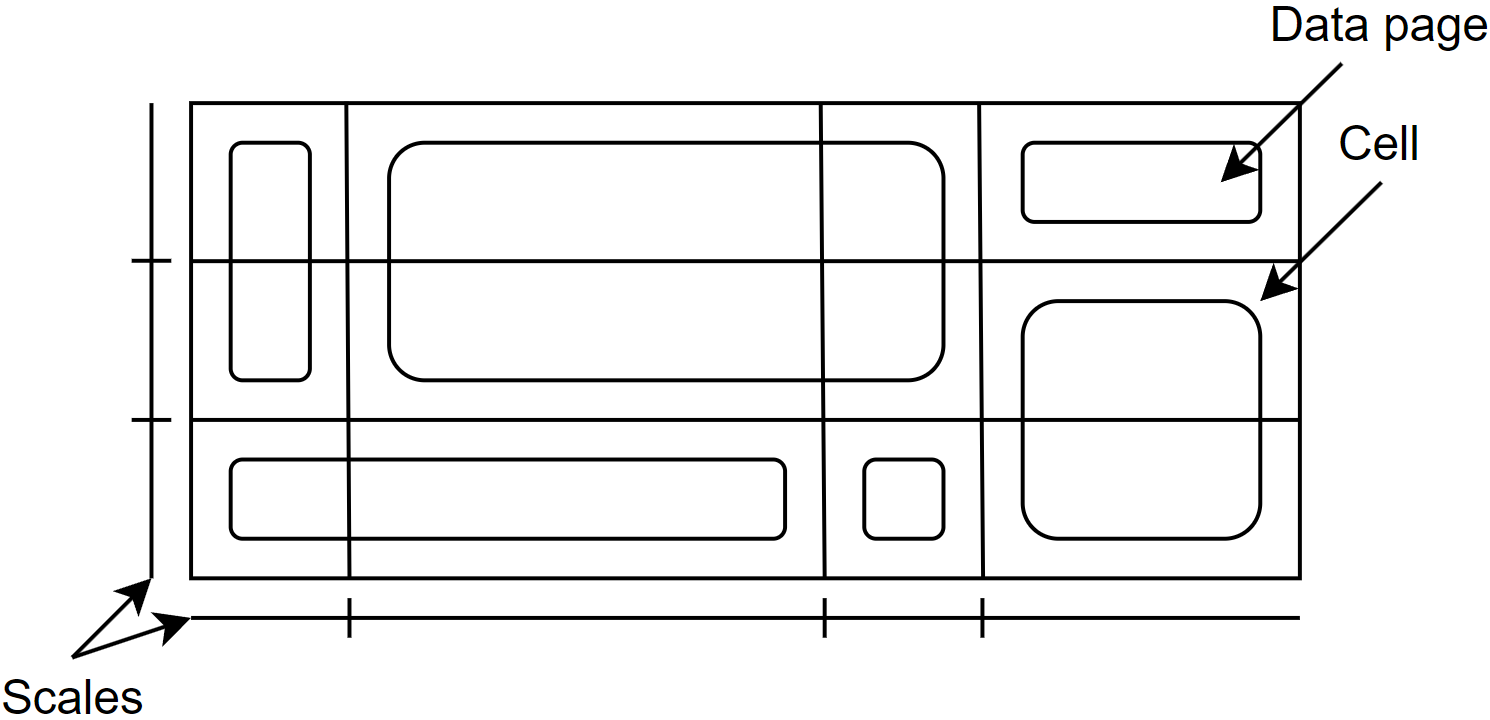
\includegraphics[width=0.5\linewidth]{images/grid.png}
\end{figure}
When a data page reaches its capacity and overflows, it undergoes a split.
After a split, the directory structure changes by applying one of the following actions: 
\begin{itemize}
    \item If the block was referenced by two or more cells, we simply update the pointers.
    \item Otherwise, if the block was referenced by a single cell, we add a separator to the directory.
\end{itemize} 
\begin{example}
    Examine the given directory:
    \begin{figure}[H]
        \centering
        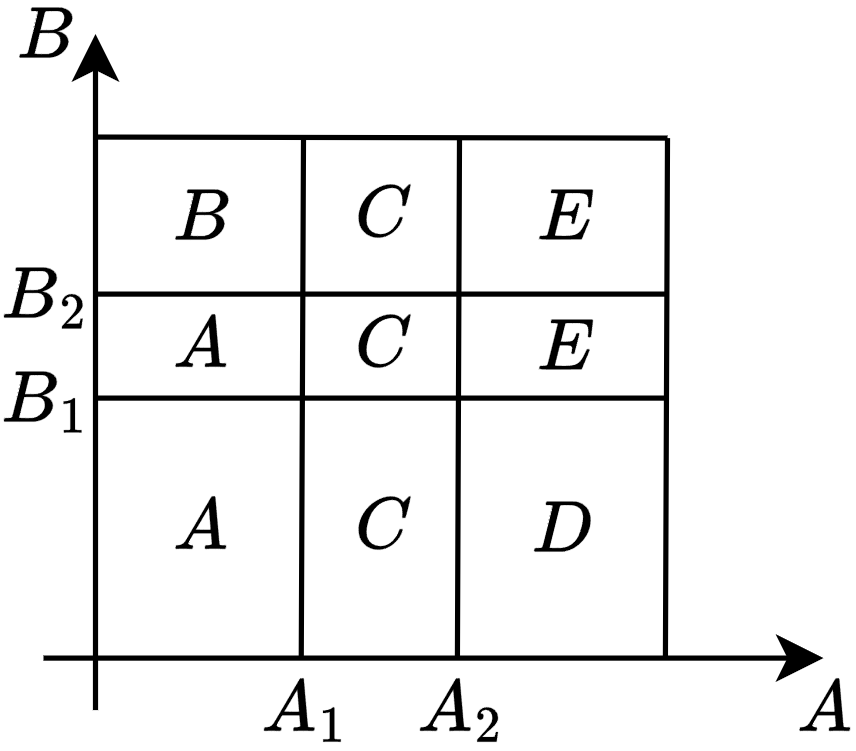
\includegraphics[width=0.25\linewidth]{images/grid1.png}
    \end{figure}
    Associated with the depicted data pages below:
    \begin{figure}[H]
        \centering
        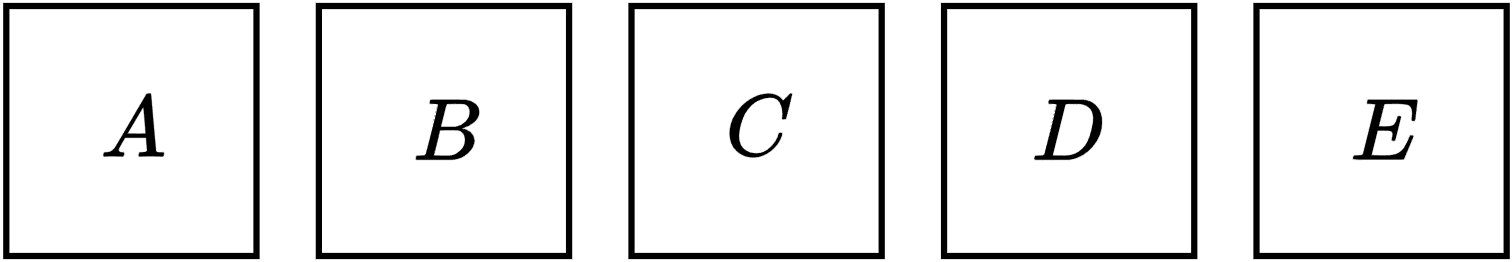
\includegraphics[width=0.4\linewidth]{images/grid2.png}
    \end{figure}
    Now, consider the scenario where $C$ overflows and undergoes a split into $C$ and $F$. 
    In this case, it is sufficient to update the pointer of the cell. 
    The resulting directory and data pages are as follows:
    \begin{figure}[H]
        \centering
        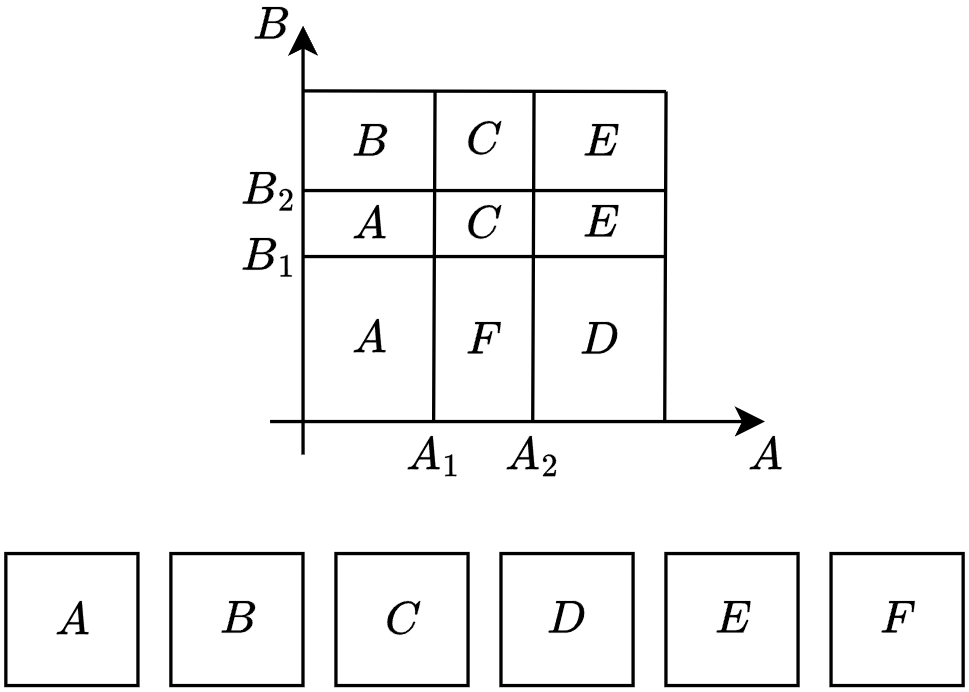
\includegraphics[width=0.5\linewidth]{images/grid3.png}
    \end{figure}
    Next, consider the case where $D$ overflows and is split into $D$ and $G$. 
    In this scenario, we need to augment the directory using an additional separator for coordinate $A$. 
    The resulting directory and data pages become:
    \begin{figure}[H]
        \centering
        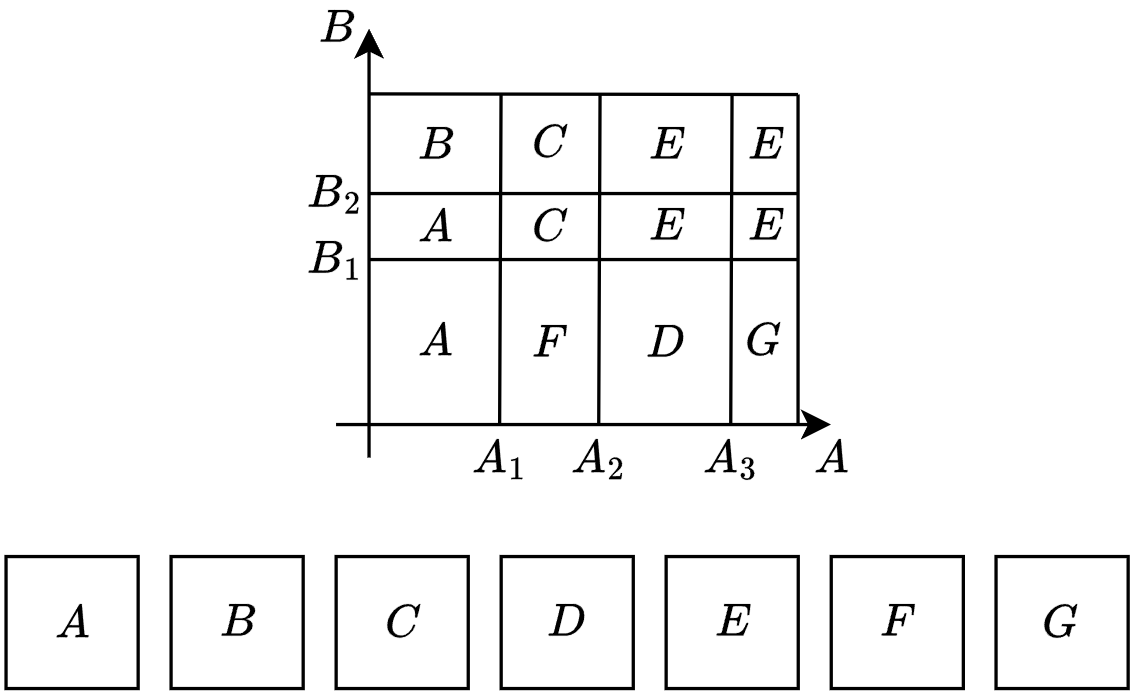
\includegraphics[width=0.6\linewidth]{images/grid4.png}
    \end{figure}
\end{example}

\paragraph*{Summary}
For non-uniform distributions, the storage of $n$ points may demand a number of cells that increases proportionally to $O(n^d)$.
In general, this approach exhibits poor performance with correlated data.
Conversely, the structured nature of space partitioning significantly simplifies the resolution of window queries.

The primary challenge with this technique lies in the management of the directory. 
Typically, scales are stored in main memory.
In quasi-static scenarios, the directory can be stored on disk as a multidimensional array.
However, in dynamic cases, it becomes essential to paginate the directory, resulting in multi-level grid files.

\subsection{R-tree}
An R-tree is a well-balanced and paginated tree structure built upon the hierarchical nesting of overlapping regions.
In this structure, every node represents a rectangular region, specifically the Minimum Bounding Box (MBB) encapsulating its children's regions.
The storage utilization for each node ranges from 100\% down to a minimum value ($\leq$ 50\%), a parameter set during design.
The management mechanisms in an R-tree bear similarities to those found in a B+ tree. 
However, a key distinction lies in the fact that the insertion of an object and splits can be handled according to different policies.

\paragraph*{Minimum Bounding Box}
The Minimum Bounding Box is the smallest rectangle containing all children regions, with sides parallel to the coordinate axes.
It is determined by the product of $d$ intervals and can be uniquely defined by the (2d) coordinates of any two opposite vertices, typically the lower-left and upper-right vertices.
The computation of the MBB for $m$ points in $d$ dimensions can be performed in $O(md)$ time.
\begin{figure}[H]
    \centering
    \includegraphics[width=0.5\linewidth]{images/MBB.png}
    \caption{Graphical representation of a 2d and a 3d MBB}
\end{figure}
The differences between a B+ tree and an R-tree are outlined below: 
\begin{table}[H]
    \centering
    \begin{tabular}{ll}
    \hline
    \multicolumn{1}{c}{\textbf{B+ tree}}                                                & \multicolumn{1}{c}{\textbf{R-tree}}                                                               \\ \hline
    Balanced and paginated tree                                                         & Balanced and paginated tree                                                                       \\
    Data are stored in leaves                                                           & Data are stored in leaves                                                                         \\
    Leaves are kept sorted and linked                                                   & No data order exist                                                                               \\
    Data are organized into 1D intervals                                                & Data are organized into d-dim intervals                                                           \\
    \makecell[l]{This principle is recursively applied \\ towards the root}             & \makecell[l]{This principle is recursively applied \\ towards the root}                           \\
    \makecell[l]{Point search follows a single path \\ from root to a single leaf}      & \makecell[l]{Point search could follow multiple paths \\ from the root to multiple leaves}        \\ \hline
    \end{tabular}
\end{table}

\paragraph*{Organization}
The R-tree is constructed by recursively aggregating objects in a bottom-up fashion, utilizing the Minimum Bounding Box (MBB). 
Overlapping regions may be present within the MBBs. 
Each node, excluding the root, has a capacity for a maximum of $C_{\text{max}}$ entries, but no fewer than $C_{\text{min}}=0.5 \cdot C_{\text{max}}$.
Visually, the structure can be represented as shown below:
\begin{figure}[H]
    \centering
    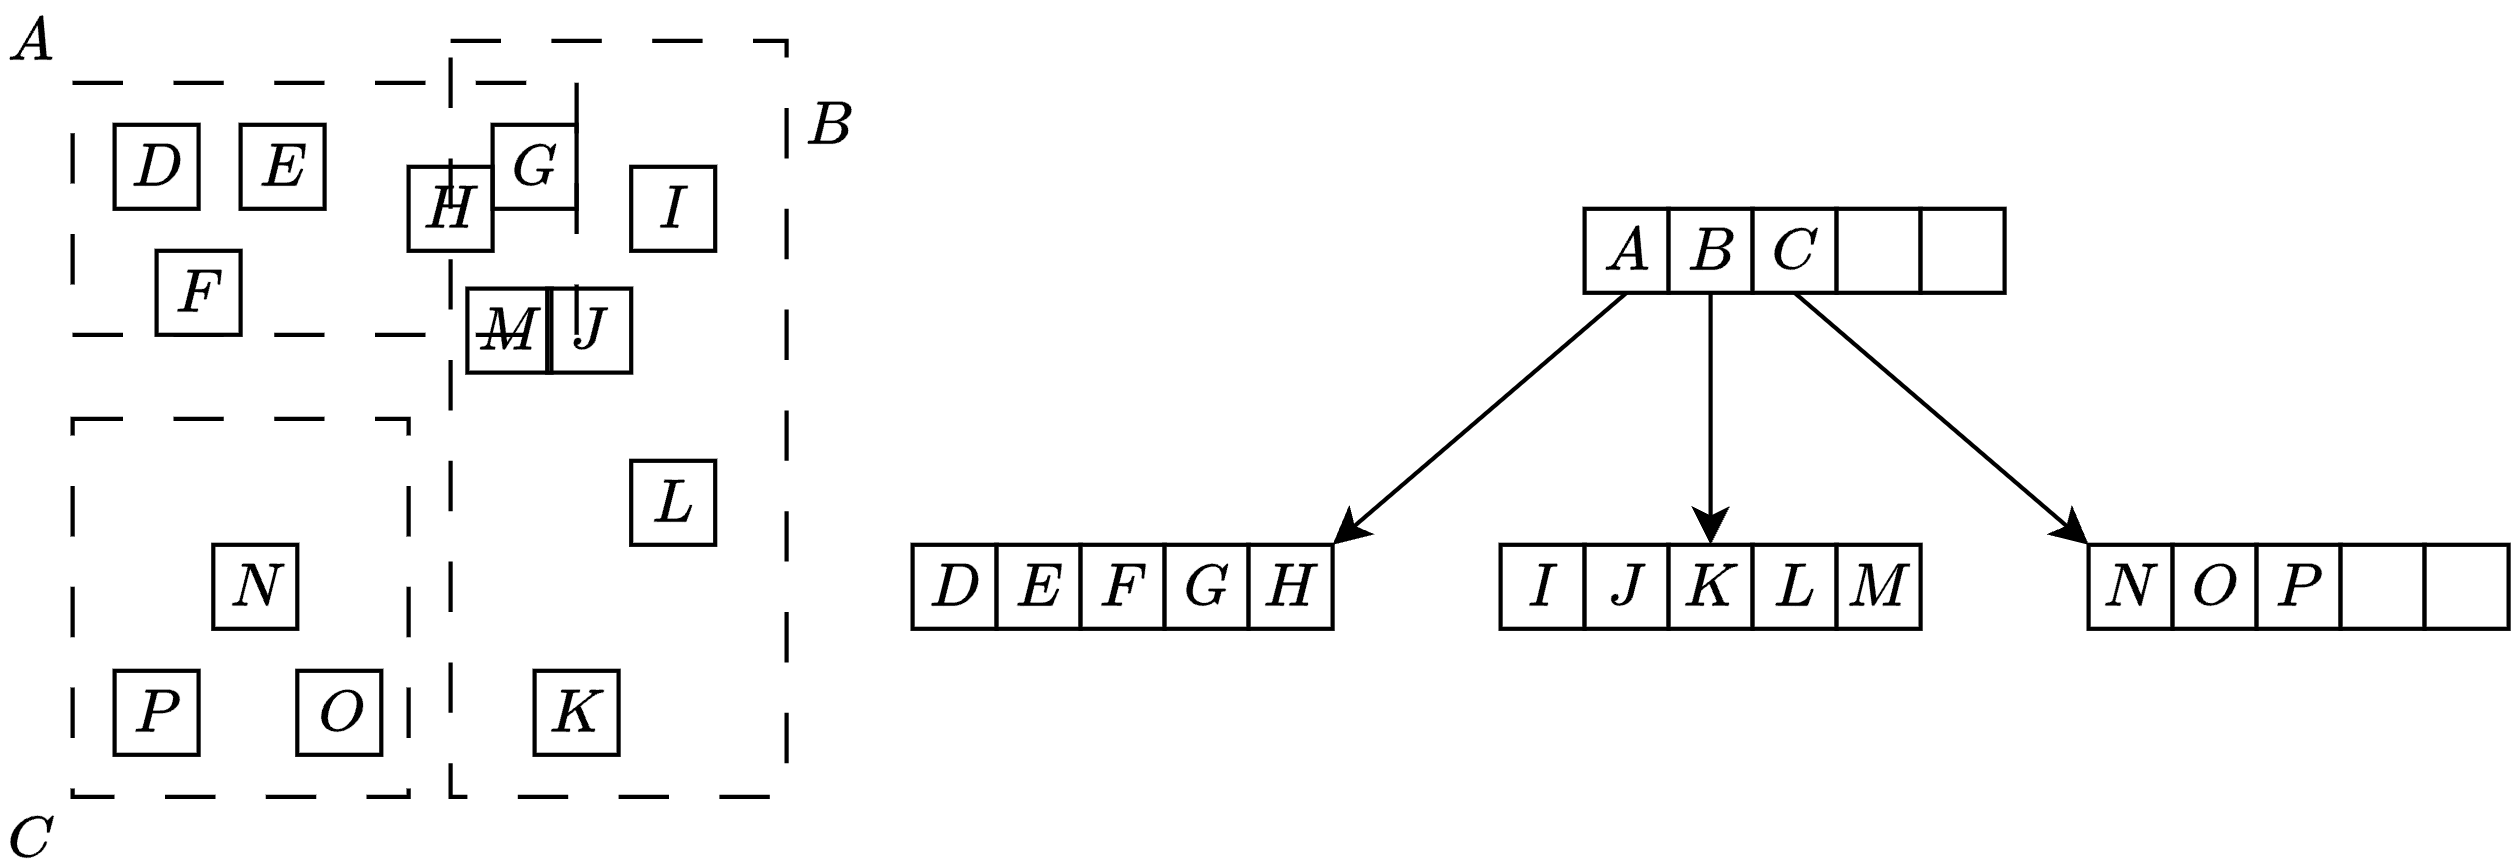
\includegraphics[width=0.75\linewidth]{images/r.png}
\end{figure}
Leaf nodes store entries in the form $\left\langle \text{key}, \text{RID} \right\rangle$, where the key holds the coordinates of the record referenced by RID.
Additionally, the R-tree is capable of storing $d$-dimensional objects with spatial extensions, where $\text{key}=\text{MBB}(\text{object})$. 

Internal nodes contain entries of the form $\left\langle \text{MBB}, \text{PID} \right\rangle$, where MBB represents the coordinates of the MBB containing all entries reachable from the node referenced by PID. 
In summary, each node contains entries in the format $\left\langle \text{key}, \text{pointer} \right\rangle$, where the key is a spatial value.

\paragraph*{Insertion}
To \texttt{insert} a new object, the process begins at the root and proceeds down the tree incrementally, seeking an optimal location to accommodate the new object $p$. 
At each step, the objective is to identify the most appropriate child node for $p$. 
In general, a penalty value is computed for each node, and the one with the minimum penalty is selected.

If point $p$ falls within the region of a node, the penalty is set to 0. 
Otherwise, the penalty is determined by the increase in volume (or area) of the Minimum Bounding Box (MBB).
For leaf nodes, the $R^{*}$ tree variant considers the increment of overlap with other regions.
Both criteria are designed to enhance tree performance, with the following considerations:
\begin{itemize}
    \item \textit{Large volume}: increases the likelihood of visiting the node during a query.
    \item \textit{Large overlap}: raises the number of nodes visited during a query.
\end{itemize}
\begin{example}
    Consider the example of inserting the point $p$ into an R-tree with nodes $A$ and $B$:
    \begin{figure}[H]
        \centering
        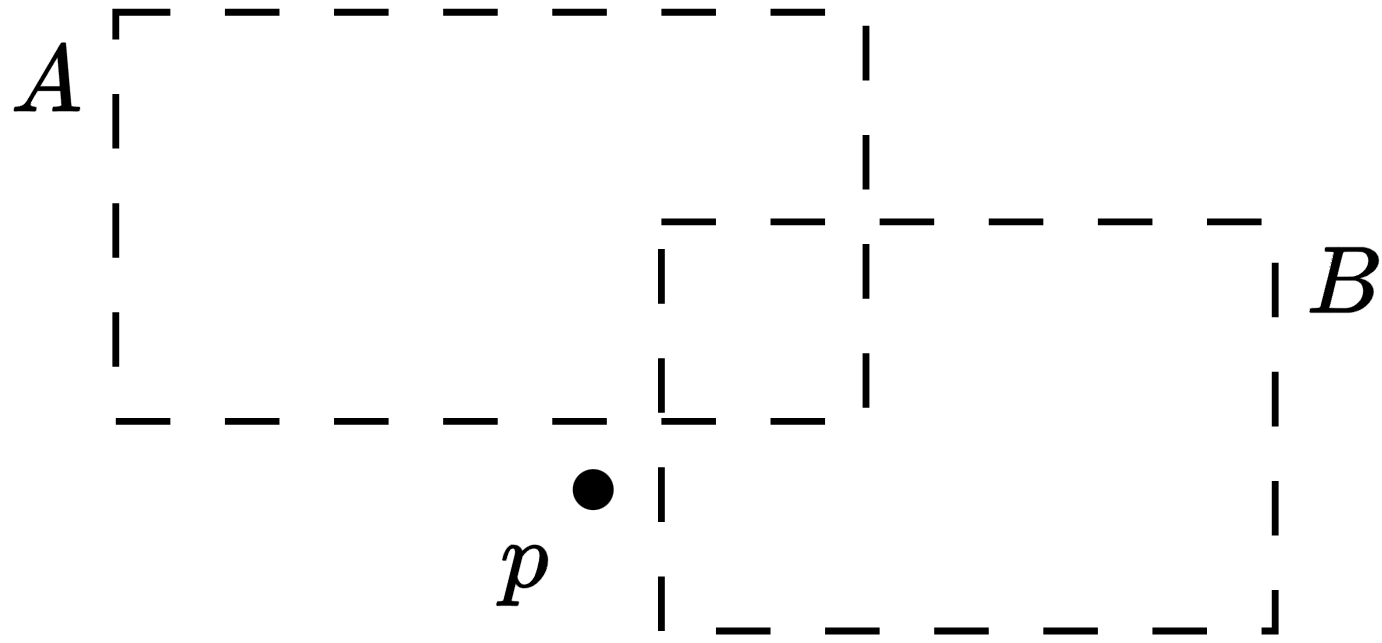
\includegraphics[width=0.4\linewidth]{images/r1.png}
    \end{figure}
    In this scenario, the most suitable area for the point $p$ is node $B$ since it results in a lower area:
    \begin{figure}[H]
        \centering
        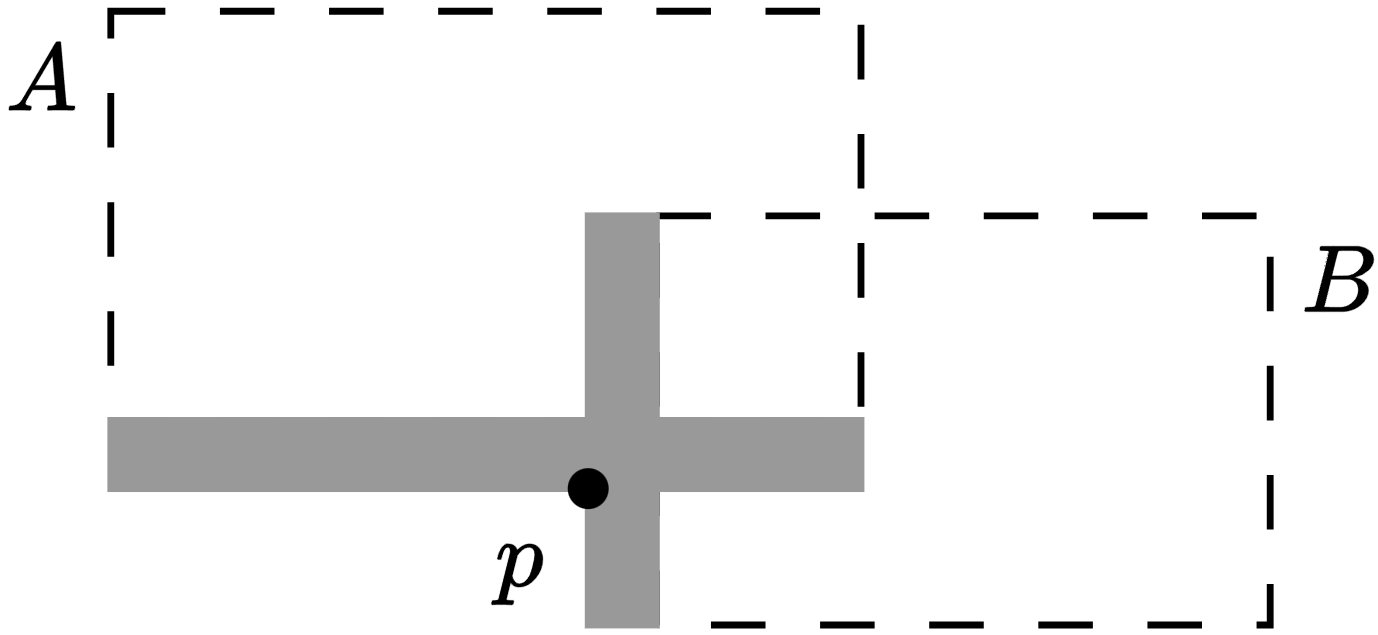
\includegraphics[width=0.4\linewidth]{images/r2.png}
    \end{figure}
\end{example}

\paragraph*{Splitting}
When the insertion of point $p$ into a leaf node $N$ results in surpassing the maximum capacity $C_{\text{max}}$, an overflow occurs, necessitating the split of node $N$.
For leaf nodes containing point entries, the goal is to divide the set of $C_{\text{max}}+1$ points into two subsets, each with a minimum of $C_{\text{min}}$ and a maximum of $C_{\text{max}}$ points.
This task is recognized as an $\mathcal{NP}$-hard problem, requiring the application of heuristics. 
Similar to B+ trees, splits propagate upward and may recursively induce splits at higher levels of the tree. 
The objective of the R-tree is to minimize the sum of resulting volumes.
In contrast, the $R^{*}$ tree employs a more intricate criterion, considering the volume, overlap, and surface of the resulting regions.
It should be noted that guaranteeing an overlap-free split is not always possible.

\paragraph*{Search}
To search for objects, we need to retrieve all points contained within the product of $d$ intervals. 
Such points are located in nodes whose Minimum Bounding Boxes (MBBs) overlap with the query region.
\begin{example}
    Consider a visual representation of a window query in the R-tree shown in the previous example:
    \begin{figure}[H]
        \centering
        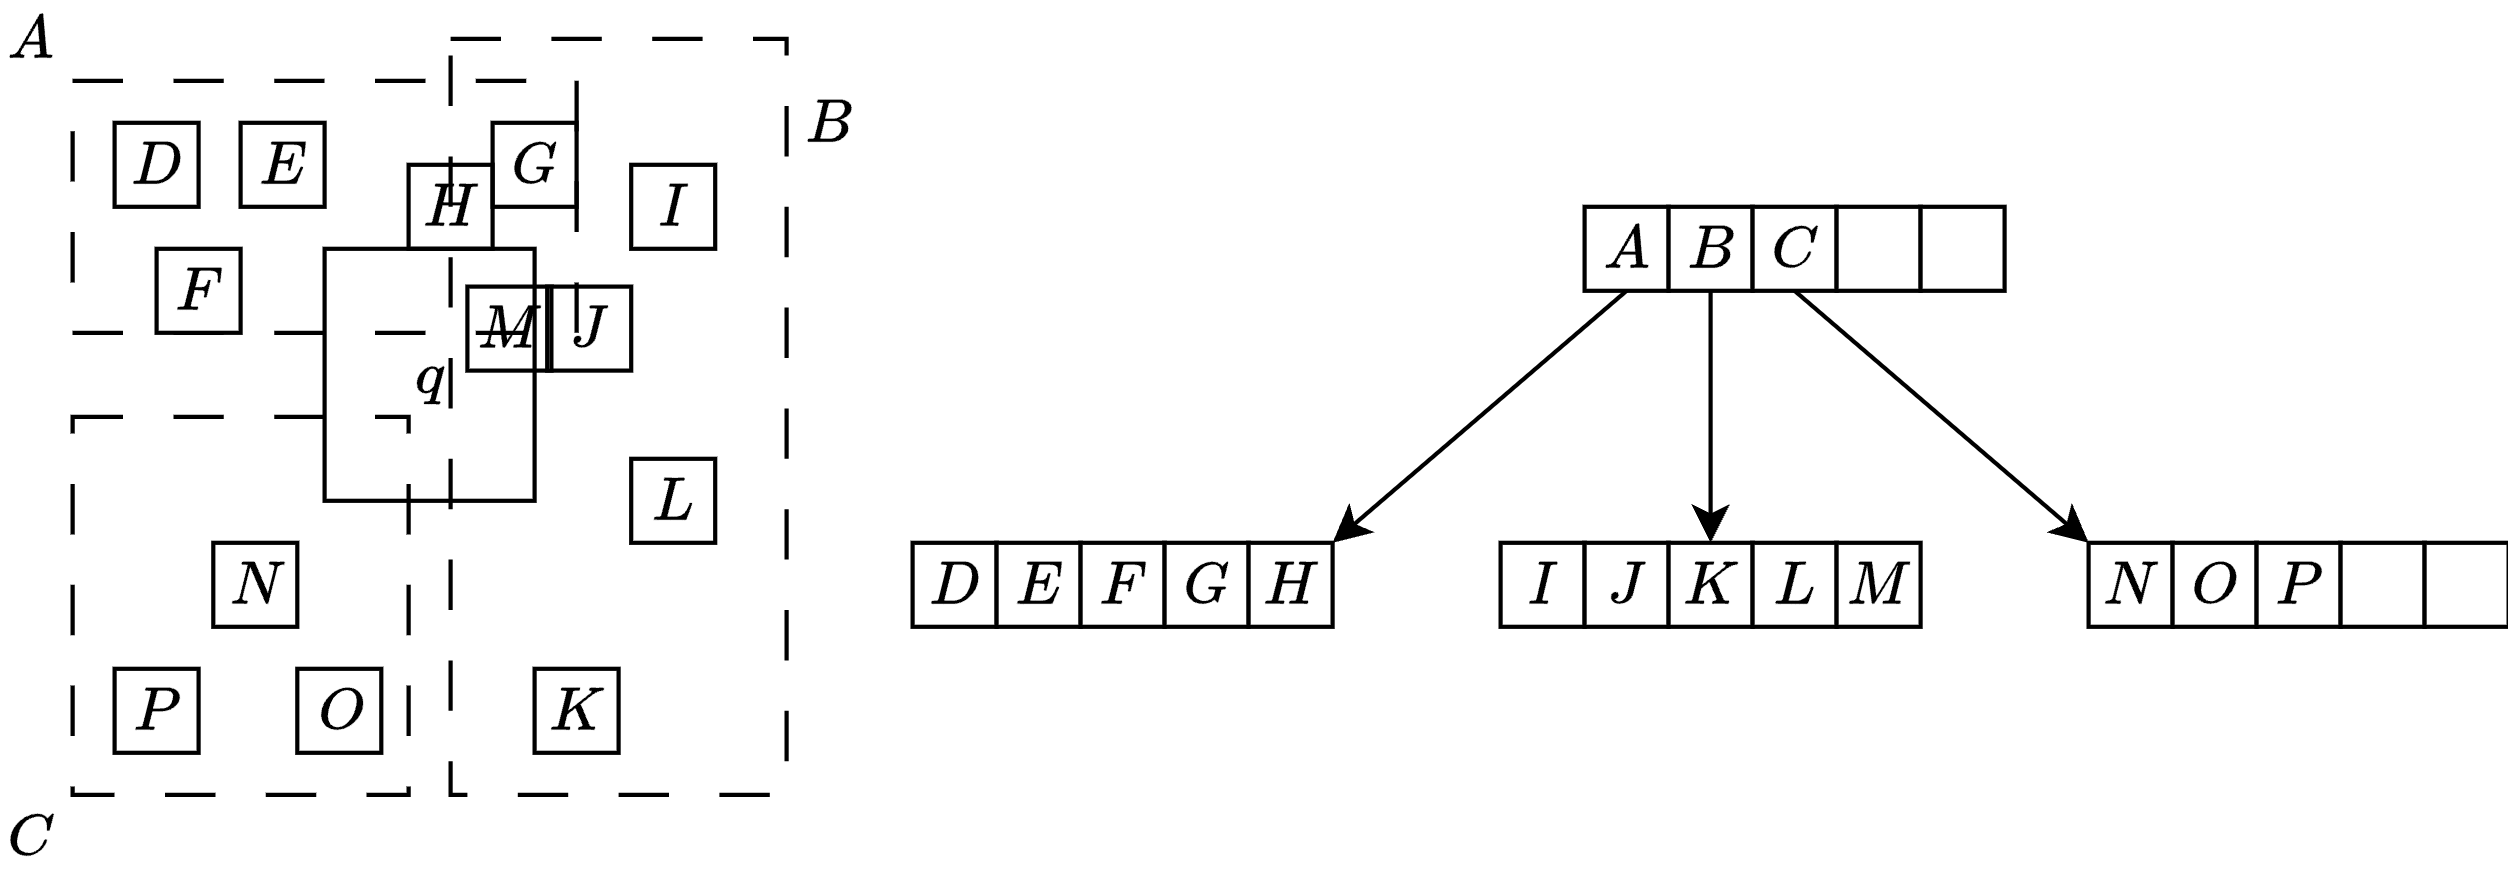
\includegraphics[width=0.75\linewidth]{images/r3.png}
    \end{figure}
\end{example}
Another type of query is the range query, which involves a query point $q$, a search radius $r$, and a distance function $D$.
The query region is defined as $\text{Reg}(q)=\{p|p \in \mathbb{R}^d, D(p,q) \leq r\}$. 
\begin{figure}[H]
    \centering
    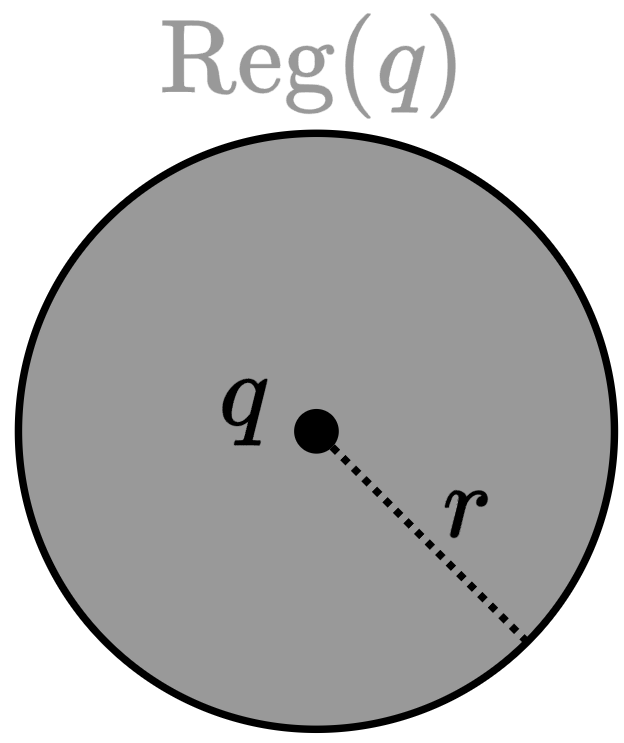
\includegraphics[width=0.15\linewidth]{images/r4.png}
\end{figure}
The algorithm for processing a range query is straightforward:
\begin{itemize}
    \item Start from the root; for each node $N$, check if MBB($N$) intersects $\text{Reg}(q)$. 
    \item On leaf nodes, for each point $p$, check if $D(p,q) \leq r$. 
\end{itemize}

\paragraph*{Search with distance functions}
For a node $N$, the minimum possible distance between the query point $q$ and a point reachable from $N$ is defined as:
\[\text{D}_{\text{MIN}}(q,N)=\inf_p\{D(q,p)|p \in \text{MBB}(N)\}\]
\begin{figure}[H]
    \centering
    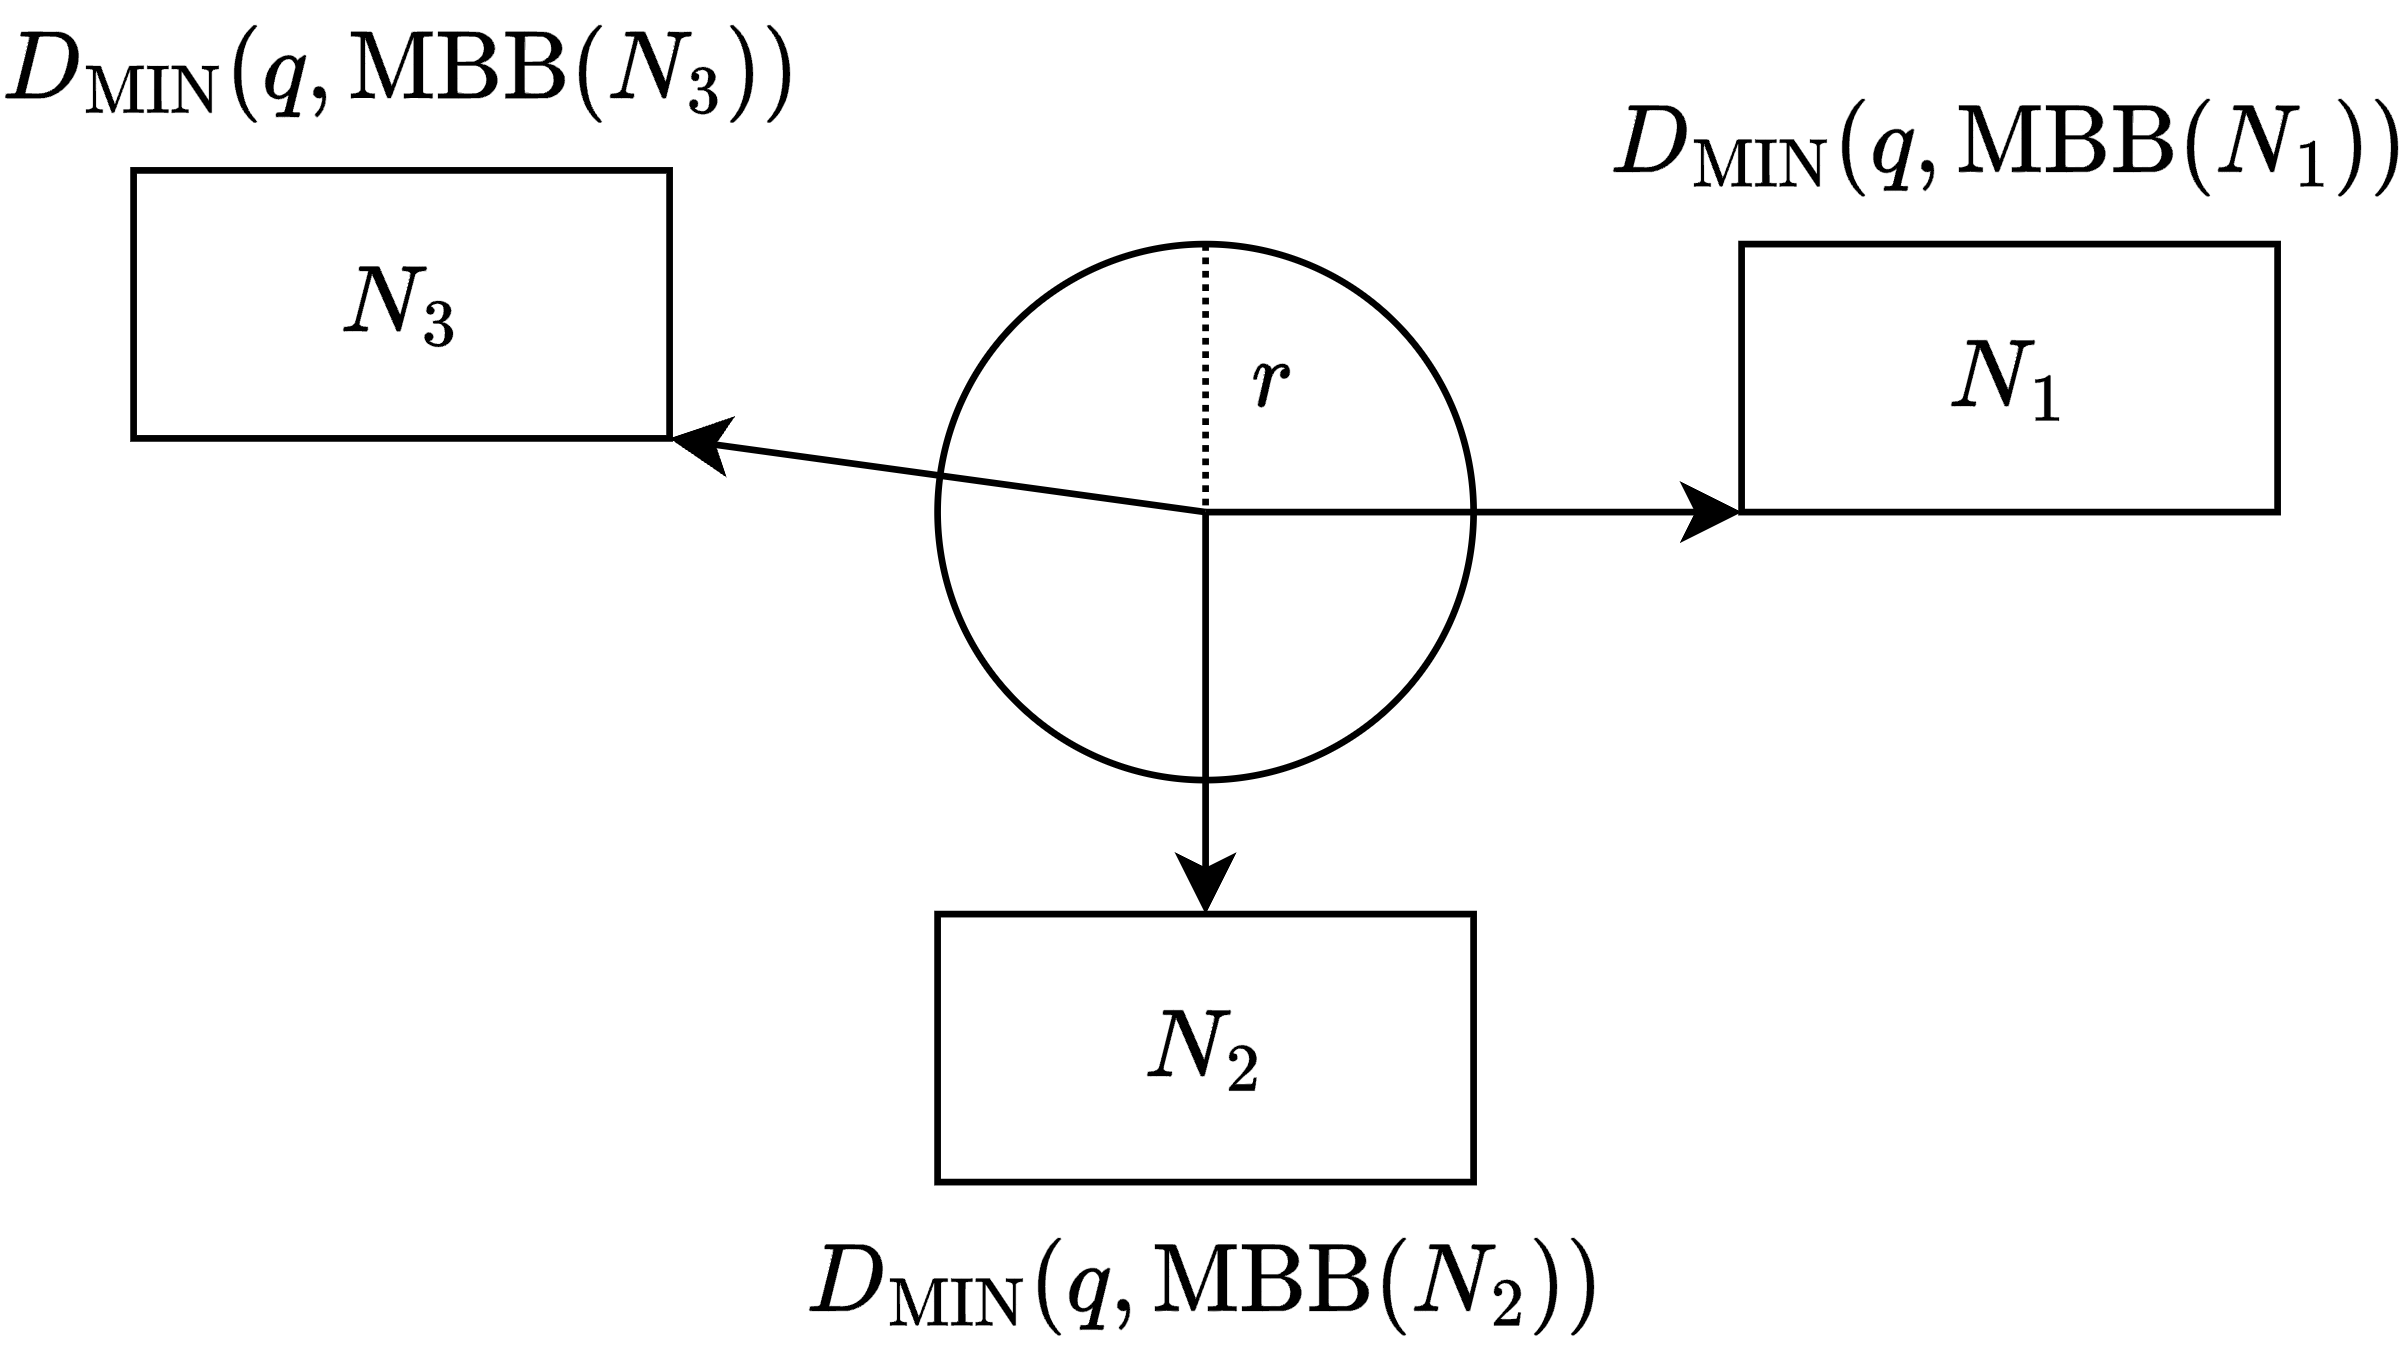
\includegraphics[width=0.5\linewidth]{images/d.png}
    \caption{Graphical representation of a general minimum distance function}
\end{figure}
The fundamental characteristic of the distance function is expressed as:
\[\text{Reg}(q) \cap \text{MBB}(N) \neq \varnothing \leftrightarrow \text{D}_{\text{MIN}}(q,N) \leq r\]
The commonly used distance functions are $L_p$-norms, generally given by:
\[L_p(t,q)=\left( \sum_{i=1}^d \left\lvert t_i-q_i \right\rvert^p  \right)^{\frac{1}{p}}\]
Notable instances of the $L_p$-norm include:
\begin{itemize}
    \item \textit{Euclidean distance}: $L_2(t,q)=\sqrt{\sum_{i=1}^{d}{\left\lvert t_i-q_i \right\rvert^{2}}}$
    \item \textit{Manhattan distance}: $L_1(t,q)=\sum_{i=1}^{d}{\left\lvert t_i-q_i \right\rvert}$
    \item \textit{Čebyšëv distance}: $L_{\infty}(t,q)=\max_{i}\{\left\lvert t_i-q_i\right\rvert\}$
\end{itemize}
These distance functions also have weighted versions:
\begin{itemize}
    \item \textit{Euclidean distance}: $L_2(t,q)=\sqrt{\sum_{i=1}^{d}{w_i\left\lvert t_i-q_i \right\rvert^{2}}}$
    \item \textit{Manhattan distance}: $L_1(t,q)=\sum_{i=1}^{d}{w_i\left\lvert t_i-q_i \right\rvert}$
    \item \textit{Čebyšëv distance}: $L_{\infty}(t,q)=\max_{i}\{w_i\left\lvert t_i-q_i\right\rvert\}$
\end{itemize}
For the $i$-th coordinate of a given Minimum Bounding Box (MBB), the offset of the query point $q=(q_1,\dots,q_d)$ with respect to $\text{MBB}(N)$ is defined as:
\[ \delta_i=\begin{cases}
    q_i-h_i \qquad \textnormal{if } q_i \geq h_i \\
    l_i-q_i \qquad \textnormal{ if } l_i \geq q_i \\
    0 \qquad\qquad \textnormal{  otherwise}
\end{cases}\]
As a result, the distance $D_{\text{MIN}}$ is computed as:
\[L_{p,\text{MIN}}(q,N;W)=\left( \sum_{i=1}^d{w_i\delta_i^p} \right)^{\frac{1}{p}}\]

\paragraph*{Search with k-NN queries}
The \texttt{kNNOptimal} algorithm provides an I/O-optimal solution for k-NN queries with an R-tree. 
The algorithm is applicable to all index structures where the region of any child node is encompassed within the region of its parent.

The fundamental case involves setting $k=1$. 
In this scenario, consider $t_{NN}$ as the first nearest neighbor of $q$ (i.e., 1-NN), with $r_{NN}=D(q,t_{NN})$ representing its distance from $q$. 
The distance $r_{NN}$ becomes known only upon the termination of the algorithm.
\begin{theorem}
    Any correct algorithm for 1-NN queries must visit at least all nodes $N$ such that $D_{\text{MIN}}(q,N) < r_{NN}$.
\end{theorem}
\begin{proof}
    If an algorithm $A$ stops by reporting a point $t$ as the $NN$ of $q$, and $A$ does not read a node $N$ such that $D_{\text{MIN}}(q,N) < D(q,t)$, then $N$ might lead to a point $t^{'}$ with $D(q,t^{'}) < D(q,t)$, contradicting the hypothesis that $t$ is the $NN$ of $q$.
\end{proof}

The \texttt{kNNOptimal} algorithm employs a priority queue PQ, consisting of pairs $\left\langle \text{ptr}(N), D_{\text{MIN}}(q,N)\right\rangle $. 
PQ is ordered based on increasing values of $D_{\text{MIN}(q,N)}$. 
Thus, \texttt{dequeue} extracts the pair with the minimum $D_{\text{MIN}}$, and \texttt{enqueue}($\left\langle \text{ptr}(N), D_{\text{MIN}}(q,MBB(N)) \right\rangle $) performs an ordered insertion of the pair into the queue.
\begin{property}
    If a point $t$ with $D(q,t) = r$ is found, then all nodes $N$ with $D_{\text{MIN}}(q,N) \geq r$ can be excluded from the search.
\end{property}
The exclusion of nodes can be achieved through pruning. 
The \texttt{update}(PQ) function facilitates this operation. 
If node pruning is not desired, the nodes can be retained in the queue until the point where further improvement in the result is unattainable.

The algorithm takes a query point $q$ and an index tree with the root node RN as input, producing outputs $t_{NN}$ (the nearest neighbor of $q$) and $r_{NN}=D(q,t_{NN})$.
\begin{algorithm}[H]
    \caption{kNNOptimal Algorithm}
        \begin{algorithmic}[1]
            \State Initialize PQ with $\left\langle \text{ptr}(RN),0 \right\rangle $
            \State $r_{NN}:=\infty$
            \While{$\text{PQ} \neq \varnothing$}
                \State $\left\langle \text{ptr}(N),D_{\text{MIN}}(q,N) \right\rangle := \texttt{dequeue}$
                \State read($N$)
                \If{$N$ is a leaf}
                    \For{each point $t \in N$} 
                        \If{$D(q,t) < r_{NN}$}
                            \State $t_{NN} := t$
                            \State $r_{NN} := D(q,t)$
                            \State \texttt{update}(PQ)
                        \EndIf
                    \EndFor
                \Else 
                    \For{each child node $N_c \in N$}
                        \If{$D_{\text{MIN}}(q,N_c) < r_{NN}$}
                            \State \texttt{enqueue}($\left\langle \text{ptr}(N_c),D_{\text{MIN}}(q,N_c) \right\rangle$)
                        \EndIf 
                    \EndFor
                \EndIf
            \EndWhile 
            \State \Return $t_{NN}$ and $r_{NN}$
        \end{algorithmic}
\end{algorithm}
The correctness of the \texttt{kNNOptimal} algorithm is evident. 
To establish its I/O-optimality, i.e., to demonstrate that it reads the minimum number of nodes, it suffices to prove the following theorem.
\begin{theorem}
    The \texttt{kNNOptimal} algorithm for 1-NN queries never reads a node $N$ whose $D_{\text{MIN}}$ is strictly larger than $r_{NN}$, i.e.: 
    \[D_{\text{MIN}}(q,N) > r_{NN}\]
\end{theorem}
\begin{proof}
    Node $N$ is read only if, at some execution step, it becomes the first element in PQ. 
    Let $N_1$ be the node containing $t_{NN}$, $N_2$ its parent node, $N_3$ the parent node of $N_2$, and so on, up to $N_h = RN$, where $h$ is the height of the tree.
    Now observe that, by definition of $D_{\text{MIN}}$, it is:
    \[r_{NN} \geq D_{\text{MIN}}(q,N_1) \geq D_{\text{MIN}}(q,N_2) \geq \dots \geq D_{\text{MIN}}(q,N_h)\]
    At each time step before we find $t_{NN}$, one (and only one) of the nodes $N_1, N_2, \dots, N_h$ is in the priority queue. 
    It follows that $N$ can never become the first element of PQ.
\end{proof}
The algorithm easily extends to the case where $k > 1$ by incorporating:
\begin{itemize}
    \item A data structure (Res), maintaining the $k$ closest objects found so far along with their distances from $q$.
    \item A current search radius, $rk$-NN, representing the distance of the current $k$-th nearest neighbor of $q$ (i.e., the $k$-th element of Res).
\end{itemize}
The remainder of the algorithm remains unchanged.

\paragraph*{Indexing regions}
Leaves can store Minimum Bounding Boxes (MBBs) of regions instead of individual points. 
Suppose the objective is to identify all data regions $o$ that are at a distance less than or equal to $r$ from the query region, expressed as $L_2(q,o) \geq r$. 
This process involves two phases:
\begin{enumerate}
    \item \textit{Filter phase}: utilize the index to retrieve all MBBs such that $L_2\left(\text{MBB}(q),\text{MBB}(o)\right) \leq r$.
    \item \textit{Refine phase}: access the actual geometries of the objects and apply the test $L_2(q,o) \leq r$.
\end{enumerate}
\begin{figure}[H]
    \centering
    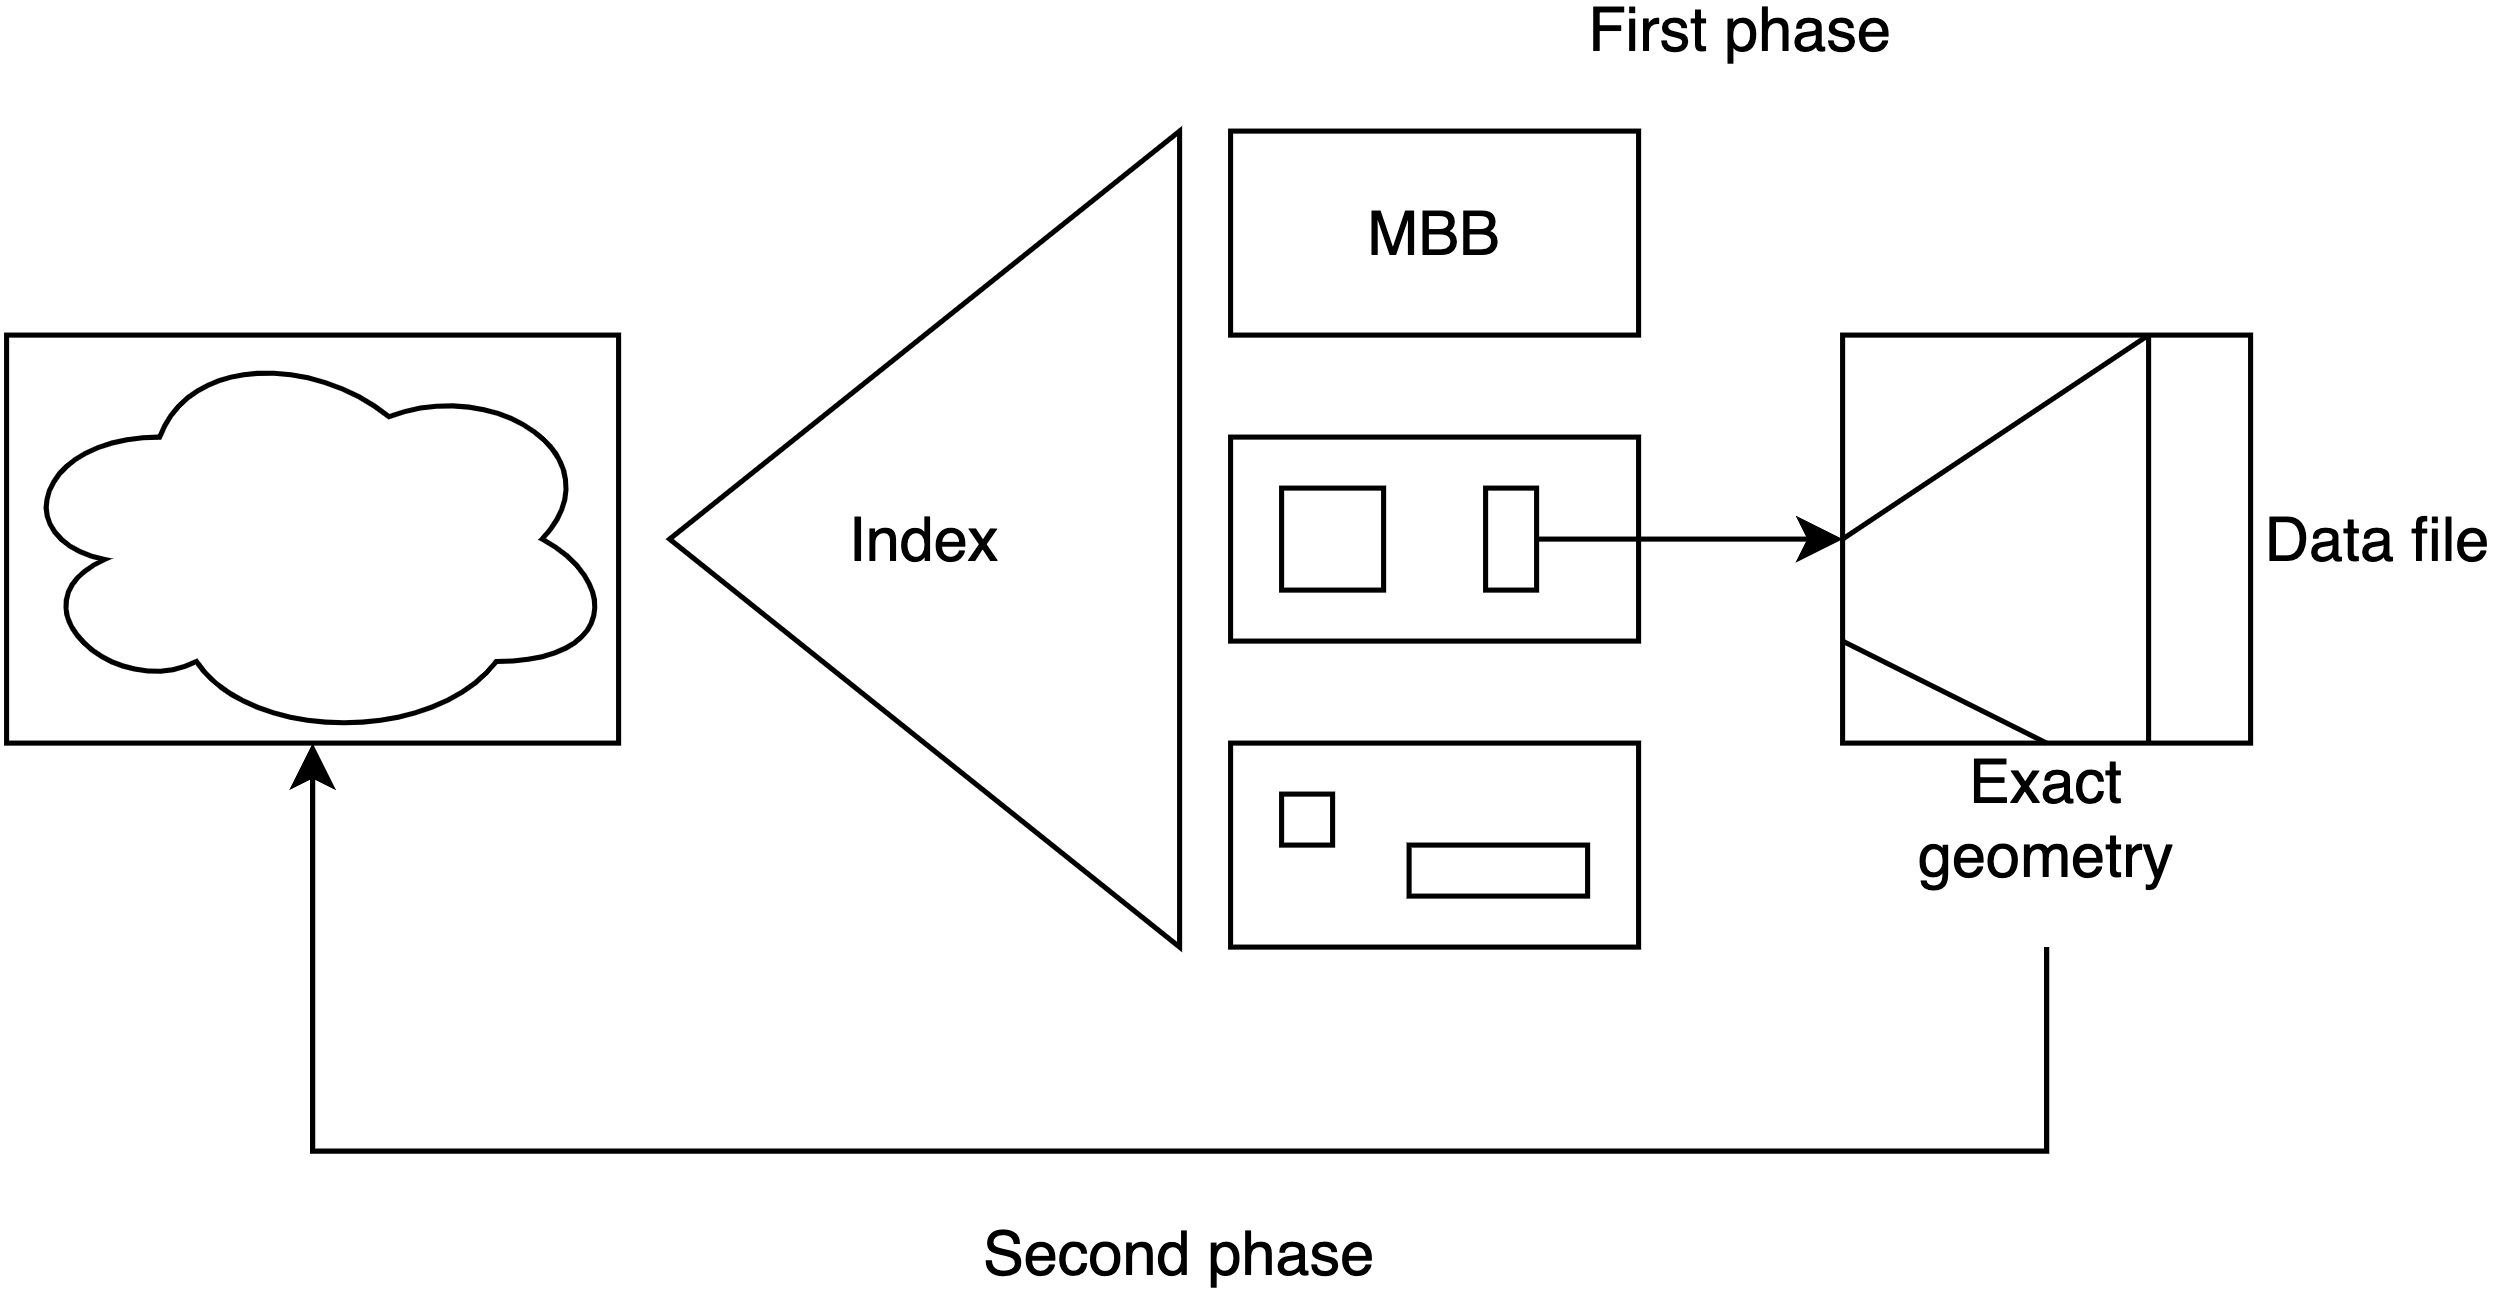
\includegraphics[width=0.75\linewidth]{images/i.png}
    \caption{Representation of indexing regions procedure}
\end{figure}